
\chapter{The Regional Arctic System Model}
\label{chap:rasm}

\section{Introduction}

I have used the Regional Arctic System Model as the main modeling tool in this dissertation.
RASM is a fully-coupled regional Earth system model (ESM) applied over a large Pan-Arctic domain (Figure \ref{fig:rasm}b).
RASM was developed under the support of the United States Department of Energy.
The development of RASM has been motivated by the need to improve multi-decadal simulations of high-latitude climate and to advance our understanding of the coupled interactions between individual components within the Arctic climate system \citep{Roberts_2010}.
RASM combines the Weather Research and Forecasting (WRF) atmospheric model \citep{Skamarock_2008,DuVivier_2016,Cassano_2016}, the Variable Infiltration Capacity (VIC) hydrology model \citep{Liang_1994,Liang_1996,Hamman_2016a}, the RVIC streamflow routing model \citep{Lohmann_1996,Hamman_2016b}, the Parallel Ocean Program (POP) model \citep{Smith_2010,Roberts_2015a}, and the Los Alamos Sea Ice (CICE) model \citep{Hunke2013,Hunke2015,Roberts_2015a} using the Community Earth System Model (CESM) coupling infrastructure \citep[CPL7; ][]{Craig_2012,Roberts_2015a}.
Additional details describing the specific application of each of the RASM component models can be found in the chapters \ref{chap:land_surface} and \ref{chap:land_surfstreamflowace} as well as in the RASM-specific literature cited above.

\begin{figure}
  \centering
  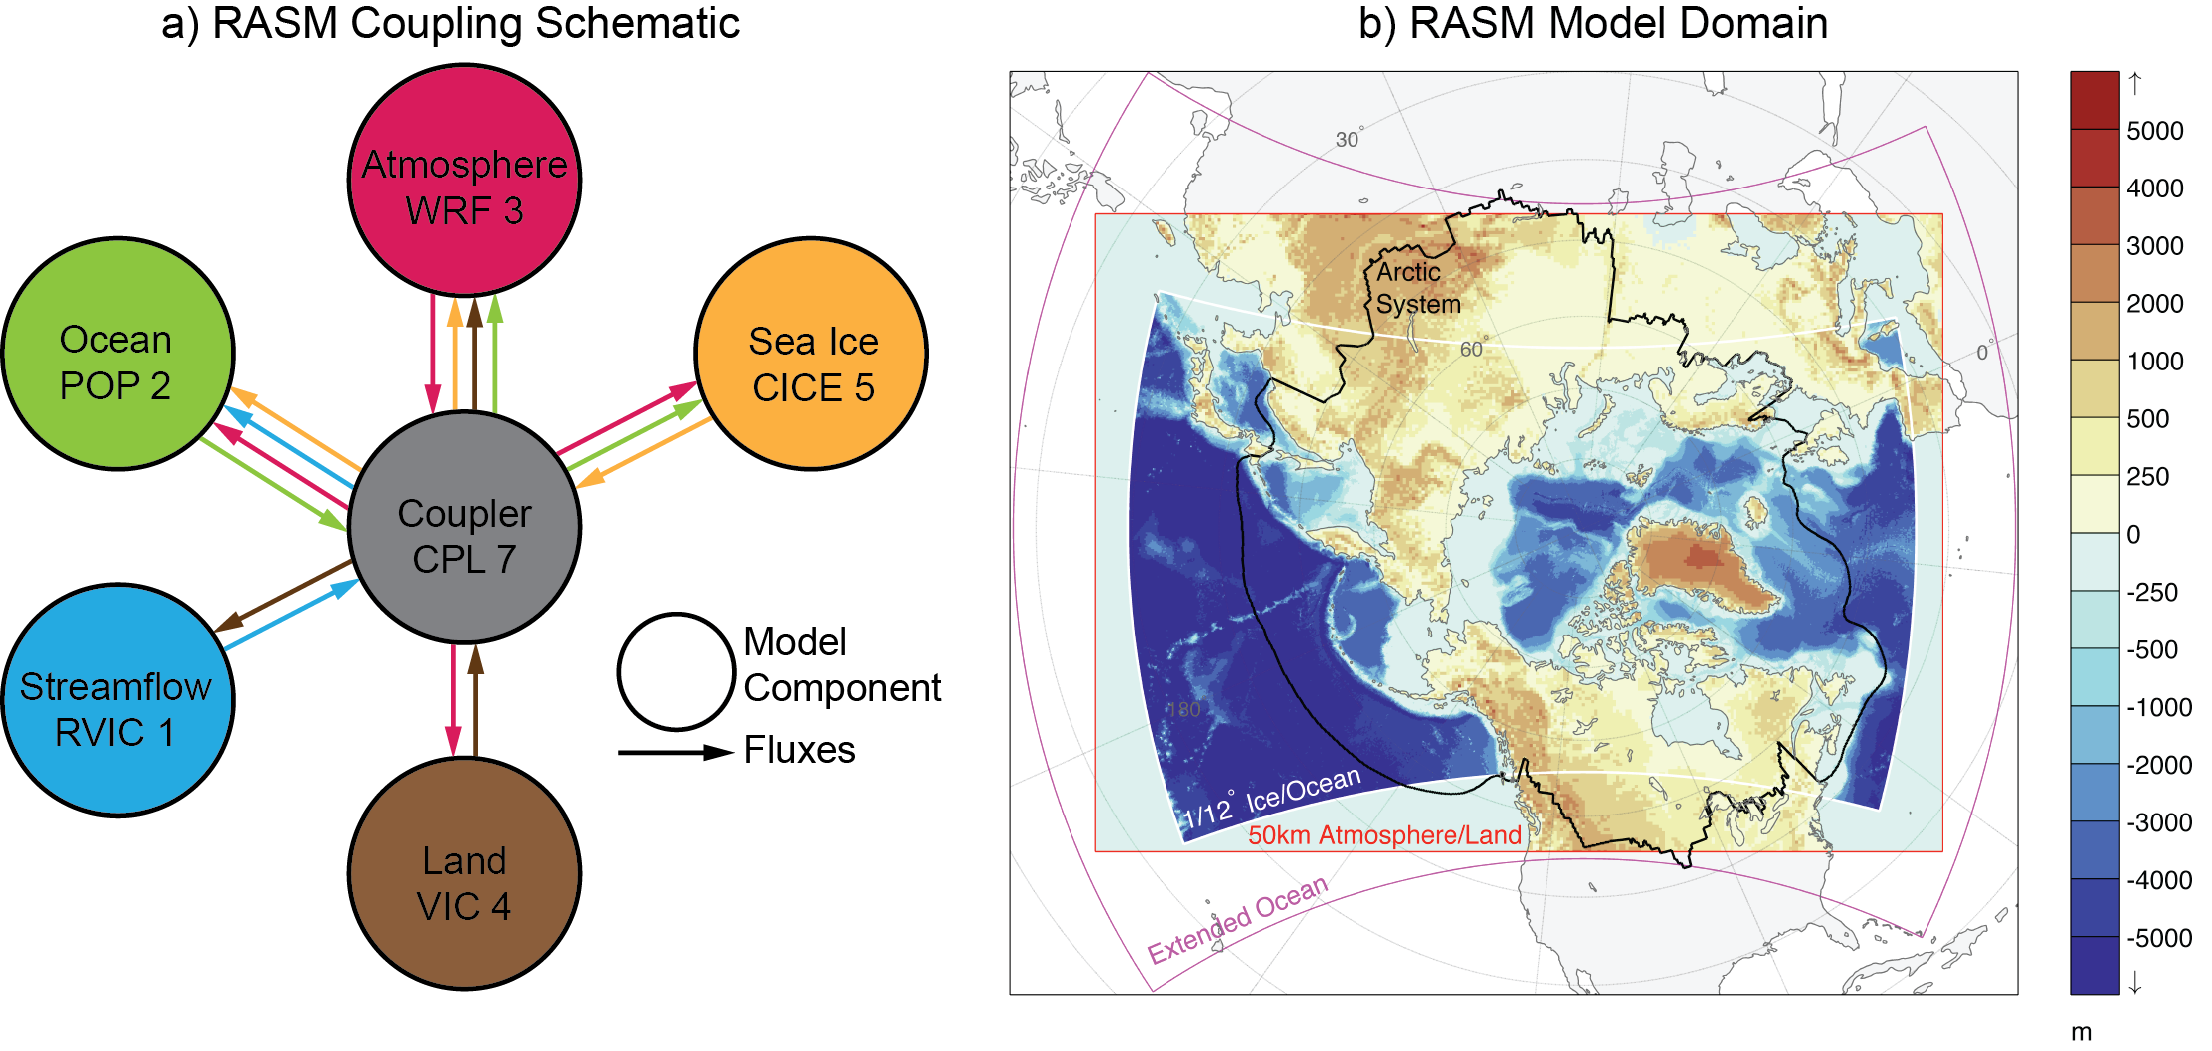
\includegraphics[width=12cm,keepaspectratio]{rasm_schematic_domain}
  \caption{a) Schematic of model configuration in RASM.
  The CPL7 flux coupler passes and receives all fluxes, shown with color coded arrows based on their source model, transferred across model boundaries.
  The component land, atmosphere, ocean, and sea ice models each calculate internal physics apart from the coupler.
  b) RASM model domain.
  There are three main grid domains in RASM, 1/12$^{\circ}$ rotated pole ice/ocean, a 50-km near equal area polar stereographic atmosphere/land/streamflow, and 1/12$^{\circ}$Extended Ocean.
  The color bar represents elevation above or below sea level.
  The black outline designates the greater Arctic Basin.}
  \label{fig:rasm}
\end{figure}

\section{Motivation}

The importance of understanding the Arctic climate system is underscored by the recent and unprecedented observed changes in key climatic processes across the region, and the potential for these changes to impact natural and human activities in coming decades.
Although it is clear that these changes are largely driven by changes in global temperature, the Arctic is expected to play an important role in modulating the rate of warming through a series of radiative, hydrologic, and biogeochemical feedbacks  \citep{Holland_2003}.
Many of the underlying processes that control these feedbacks are either poorly or under represented in global models, which often leads to the misrepresentation the true feedback sensitivity.
global models poorly represent some processes (sea ice, permafrost, runoff, precipitation, circulation)
The development of RASM is motivated by the need to better represent a range of regional processes (e.g. sea ice, permafrost, ice sheets) and feedbacks (e.g. ice-albedo feedback, biogeochemical feedbacks related to permafrost).
RASM seeks to improve the representation of a range of high-resolution processes unique to the polar regions and to provide improved understanding of the coupled relationship between climate system components.

The development and use of a regional climate model, such as RASM, has advantages and disadvantages when compared to global climate model (GCMs).
Most notably, from a computational perspective, regional models are applied over a smaller region than global models, they may be run at higher spatial and temporal resolutions.
Higher resolution is generally thought to improve model representation of certain processes, such as orographic precipitation, coastal processes, and mesoscale processes \citep{Feser_2011}.
Another way to think of how high-resolution regional models are useful is as a ``testbed'' for future global model parameterizations.
As global models trend to higher resolutions, parameterizations related to model dynamics (e.g. ocean eddies, clouds, convective precipitation) will need to be re-evaluated; regional models offer a way to test out new combinations of parameterizations \citep[e.g. ][]{Roberts_2015a,Cassano_2016}.
Regional models must be forced at their lateral boundaries with output from a global model (either reanalysis or a GCM).
In some cases, this can be viewed as a disadvantage of using a regional model since global climate feedbacks are not accounted for.
Conversely, forcing regional models at their boundaries limit the degrees of freedom in the climate system, which can be viewed as an advantage when interpreting the response of new model parameterizations.

\section{Application}

The RASM domain includes the entire Arctic drainage basin and encompasses the historical extent of seasonal sea ice cover.
For the work presented in this dissertation, the land, atmosphere, and runoff components in RASM are applied over a 50-km near equal-area stereographic grid, while the ocean and sea ice components are applied over a $1/12^{\circ}$ rotated sphere mesh (Figure \ref{fig:rasm}b).
The individual model components (Figure \ref{fig:rasm}a) in RASM are tightly-coupled in RASM, exchanging flux variables though the flux coupler every 20 minutes.
This coupling configuration is described by \citet{Roberts_2015a}, where the sub-daily coupling frequency is shown to be important in reproducing observed inertial frequencies in the atmosphere-ice-ocean coupling cycle.

RASM version 1.0 was completed in 2015 and since then it has been used in a range of applications.
\citet{Roberts_2015a} used RASM to develop refined ice-ocean-atmosphere coupling scheme for sub-hourly timesteps.
They went on to show how this improvement leads to better simulation of inertial oscillations and semi-diurnal sea ice drift in RASM and in a CESM.
This paper is a good example of how RASM can be used as a testbed for high-resolution climate modeling.
RASM was used by \citet{DuVivier_2016} to evaluate characteristic patterns of atmosphere-ocean coupling resulting from strong winds along the southeast Greenland coast.
\citet{Cassano_2016} used RASM to evaluate a range of sea ice, ocean, and atmospheric parameterizations in terms of their impact on radiation biases.
This paper has motivated the upgrade and extension of the WRF model within RASM to improve known biases in WRF's radiation and microphysics schemes, work that is currently underway.
This dissertation (Chapters \ref{chap:land_surface}, \ref{chap:streamflow}, and \ref{chap:winter_prec}) represent the existing body of work related to the development and evaluation of the land surface within RASM.
